%!TEX root = etdrtemplate.tex
% +--------------------------------------------------------------------+
% | Chapter 3
% +--------------------------------------------------------------------+

\cleardoublepage

% +--------------------------------------------------------------------+
% | Replace "This is Chapter 3" below with the title of your chapter.
% | LaTeX will automatically number the chapters.
% +--------------------------------------------------------------------+

\chapter{PCA Pump Prototype}
\label{pcapump}

Overview of PCA Pump and issues, which MDCF/ICE will solve.
%http://ppahs.org/2012/05/30/patient-controlled-analgesia-pca-pumps-the-basics/
In this thesis, only the operation module is implemented.
Overview of Safety-Critical System loop.

\begin{figure}[ht]%t=top, b=bottom, h=here
    \begin{center}
    	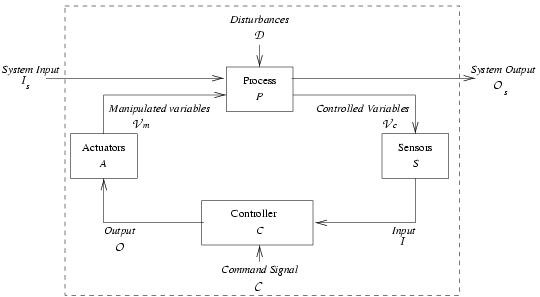
\includegraphics[height=3.5in]{figures/safety-critical-loop.png}
    	\caption{Basic Process Control Loop\protect\footnotemark.}
    \end{center}
\end{figure}
\footnotetext{http://www.safeware-eng.com/system and software safety publications/Designing Specification Languages.htm}

Pump internal implementation based on \cite{CADD-PrizmAmbulatoryInfusionPump:Online}.
- basal dose deliver in increments - easier to track delivered amount (page 14)


\section{PCA Pump Requirements Document}
\label{pcapump:requirements-doc}

Selected use cases for implementation?

%state machine image

Overview of issues solved: 
* Bolus options: FBasal + FPatient or FPatient => implemented: FBasal + FPatient (consistent in doc)
5 modes:
* Stopped: F=0
* KVO: F=0.1
* Basal: F=Fbasal
* Patient: F = Fbasal + Fbolus (for vtbi/Fbolus)
* Clinician: F = Fbalsal + Fbolus (for specified time)

Most common Examiner\cite{Examiner:Online} erroes/warnings:
***        Warning                     :302: This expression may be
***        Semantic Error              :725: Protected function or variable XXX may only appear directly in an assignment or return statement.


\section{PCA Pump AADL/BLESS Models}
\label{pcapump:aadl-bless-models}
Selected modules for implementation. Pictures etc.


\section{BeagleBoard-XM}
\label{pcapump:beagleboard}
First step was create PCA Pump prototype on BeagleBoard-xM.

BeagleBoard-xM is Embedded device with AM37x 1GHz ARM processor (Cortex-A8 compatible). It has 512 MB RAM, 4 USB 2.0 ports, HDMI port, 28 General-purpose input/output (GPIO) ports and Linux Operating System (on microSD card). Moreover there is PWM support. All these properties makes this device good candidate for prototyping PCA Pump.

Pulse width modulation (PWM) is a technique for controlling analog circuits with a processor's digital outputs.

Expansion port 14(PWM) and 28(GND?)
GPIO158
Java Program to Run the pump for 10 seconds

There is no existing SPARK Ada compiler running on ARM system. Hence, to compile SPARK Ada program for ARM device, we need to perform cross-compilation on other machine. There is GNAT compiler \cite{Horn:Thesis} created by AdaCore, but there was no cross-compiler for ARM. However AdaCore was working on it. They had working version in 2013, but tested only on their target, Android-based device. BeagleBoard-xM is coming with Linux Angstrom Operating System. There is possibility to install Android on BeagleBoard-xM, but still not warranty everything will be working. Cooperation with AdaCore allowed to cross-compile SPARK Ada program for BeagleBoard-xM.

Include source of simple program?
GNAT cross-compiler only for Linux Platform (cross-compilation has to be done on Linux).

compilation+linking command: \lstinline{arm-linux-gnueabi-gnatmake -d -Ppca_ravenscar.gpr}.

%describe how to run the program: compile cmd with arm-gnuaebi... then copy to the board etc.

